\documentclass{article}

\usepackage{arxiv}

\usepackage[utf8]{inputenc} % allow utf-8 input
\usepackage[T1]{fontenc}    % use 8-bit T1 fonts
\usepackage{lmodern}        % https://github.com/rstudio/rticles/issues/343
\usepackage{hyperref}       % hyperlinks
\usepackage{url}            % simple URL typesetting
\usepackage{booktabs}       % professional-quality tables
\usepackage{amsfonts}       % blackboard math symbols
\usepackage{nicefrac}       % compact symbols for 1/2, etc.
\usepackage{microtype}      % microtypography
\usepackage{graphicx}

\title{Spatial Analysis For Class Arachnida}

\author{
    Nyx Zhang
   \\
     \\
   \\
  \texttt{} \\
   \And
    Tia Wang
   \\
     \\
   \\
  \texttt{} \\
   \And
    Yuhong Chen
   \\
     \\
   \\
  \texttt{} \\
  }


% tightlist command for lists without linebreak
\providecommand{\tightlist}{%
  \setlength{\itemsep}{0pt}\setlength{\parskip}{0pt}}


% Pandoc citation processing
\newlength{\cslhangindent}
\setlength{\cslhangindent}{1.5em}
\newlength{\csllabelwidth}
\setlength{\csllabelwidth}{3em}
\newlength{\cslentryspacingunit} % times entry-spacing
\setlength{\cslentryspacingunit}{\parskip}
% for Pandoc 2.8 to 2.10.1
\newenvironment{cslreferences}%
  {}%
  {\par}
% For Pandoc 2.11+
\newenvironment{CSLReferences}[2] % #1 hanging-ident, #2 entry spacing
 {% don't indent paragraphs
  \setlength{\parindent}{0pt}
  % turn on hanging indent if param 1 is 1
  \ifodd #1
  \let\oldpar\par
  \def\par{\hangindent=\cslhangindent\oldpar}
  \fi
  % set entry spacing
  \setlength{\parskip}{#2\cslentryspacingunit}
 }%
 {}
\usepackage{calc}
\newcommand{\CSLBlock}[1]{#1\hfill\break}
\newcommand{\CSLLeftMargin}[1]{\parbox[t]{\csllabelwidth}{#1}}
\newcommand{\CSLRightInline}[1]{\parbox[t]{\linewidth - \csllabelwidth}{#1}\break}
\newcommand{\CSLIndent}[1]{\hspace{\cslhangindent}#1}

\begin{document}
\maketitle


\begin{abstract}
This paper will examine the spatial first and second moment
characteristics of Arachnida distribution in British Columbia and
construct a Poisson Process model to forecast point distribution. We
will classify the Araneae and Opiliones orders as groups to create
visualizations that provide us with additional information about the
Arachnida subgroups.
\end{abstract}


\hypertarget{introduction}{%
\section*{Introduction}\label{introduction}}
\addcontentsline{toc}{section}{Introduction}

Arachnida (Figure \ref{fig:fig1}) is a class of joint-legged
invertebrates that includes spiders, scorpions, ticks, mites, and other
similar organisms. Arachnids play important roles in ecosystems, as well
as in human culture and mythology. Some species, like spiders, are
important for controlling insect populations, while others, like ticks,
can transmit diseases. Many arachnids have also been used in traditional
medicine, and some are kept as pets or used in scientific research. (see
Wikipedia (2023a))

Many of Arachnids are predators, using their venom and other adaptations
to capture and kill prey. Others are scavengers, feeding on dead animals
and plant material, or parasites, living on or within other organisms.
Arachnids are found in almost every habitat, from forests to deserts to
aquatic environments.

Arachnids are classified into two major orders, namely Araneae
(Wikipedia (2023b)) and Opiliones (Wikipedia (2023c)). While Araneae or
spiders are popular, Opiliones or ``harvestmen'' are not as familiar.
The main physiological differences between them are the presence of
venom-producing glands and their feeding habits. Spiders produce venom
to liquefy their food, while Opiliones lack venom-producing glands and
depend on chewing to consume their food.

Understanding their spatial distribution can provide insights into their
habitat requirements, ecological niche, and interactions with other
organisms in the ecosystem. Spatial analysis can be used to identify
areas of high arachnid diversity and conservation value. In addition, it
can help to identify areas where they may come into contact with humans,
and where there may be a risk of disease transmission or other negative
interactions.

This paper will examine the spatial characteristics of Arachnida
distribution in British Columbia and construct a Poisson Process model
to forecast point distribution. We will classify the Araneae and
Opiliones orders as groups to create visualizations that provide us with
additional information about the Arachnida subgroups.

We will obtain our data from the Global Biodiversity Information
Facility (GBIF), which offers various species distribution data
worldwide. Specifically, we will use the Spencer Entomological Museum
(Spencer (2023)) and filter the class to Arachnida and the province to
BC. We reprojected the coordinates from Lat Long, to BC Albers
projection. The final data has the size of 749 rows and 50 columns,
where Araneae accounts 675 occurrences of and Opiliones accounts 74. The
main information is the variety of the species, as well as the occurred
coordinates and dates. Human Footprint Index (HFI), Forest cover,
Distance to Water (Dist\_Water), and Elevation will be used as
additional information to analyze the covariance effects.

We will mainly examine the intensity, clustering and covariates
characteristics, based on which a model will be constructed to estimate
the intensity of Arachnida.

\hypertarget{methods}{%
\section*{Methods}\label{methods}}
\addcontentsline{toc}{section}{Methods}

The First Moment Descriptives includes measures that describe the center
or location of the spatial data distribution. This includes the mean,
median, and mode. In this study, intensity as the mean will be focused
on, which represents the average value of Arachnida density across the
study area. These measures provide insights into the central tendency of
Arachnida density in the study area.

The Second Moment Descriptives includes measures that describe the
clustering effect of the Arachnida density distribution in the study
area. This Morisita's Index should be close to 1 if points are
independent of one another, lower than 1 if there is avoidance, and
greater than 1 if there is attraction. Ripley's K function, which is a
function of the area of a circle with radius r. Any deviations between
the empirical and theoretical K-functions can show an indication of
correlations between points. The Pair Correlation Function is a
statistical method used in spatial analysis to measure the degree of
clustering or dispersion of objects in a spatial point pattern. The PCF
compares the observed distribution of objects with the distribution that
would be expected if the objects were randomly distributed, and computes
a summary statistic that reflects the degree of clustering or
dispersion. Under Complete Spatial Randomness (CSR), pair correlation
function has an expected value of 1, values \textless1 indicate fewer
points with separation distance r than expected (i.e.~avoidance), and
vice versa for function \textgreater1. These measures provide insights
into the degree of variability in Arachnida density across the study
area.

Model based on poisson point process based on examined covariates, which
is a stochastic process used to model the random locations of events in
space or time. The Poisson distribution is used to model the probability
of the number of events occurring in a given space or time interval,
assuming that the events are independent and the rate of occurrence is
constant. The PPP is characterized by a single parameter, lambda, which
represents the expected number of events in a given space or time
interval. The probability of observing k events in the interval is given
by the Poisson distribution with mean lambda.

\hypertarget{results}{%
\section*{Results}\label{results}}
\addcontentsline{toc}{section}{Results}

\hypertarget{descriptive-statistics}{%
\subsection*{Descriptive Statistics}\label{descriptive-statistics}}
\addcontentsline{toc}{subsection}{Descriptive Statistics}

From Figure \ref{fig:descrb}, we can see, in 1982, there is a
substantial increase in the number of recorded Araneae occurrences,
which may suggest potential measurement bias, thus affecting the
confidence in the absolute numbers or proportions. Nevertheless, by
examining the trendline over the years, it can still be inferred that
Araneae are more abundant than Opiliones in the region. Various factors
could contribute to this disparity, such as differences in habitat
preferences, population sizes, or environmental conditions.

Orders in the Araneae family that contribute more than 5\% to the total
Arachnida class include Lycosidae (26.97\%), Gnaphosidae (17.62\%),
Theridiidae (7.74\%), Salticidae (7.21\%), and Thomisidae (6.81\%). In
the case of the Opiliones order, only the Phalangiidae family reaches a
proportion above 5\%, accounting for 7.61\% of the total class.

\begin{itemize}
\tightlist
\item
  Intensity
\end{itemize}

Araneae has a higher intensity (7.118283e-10) compared to both Opiliones
(7.803747e-11) and the overall Arachnida class (7.803747e-11). This
means that Araneae are more densely distributed or concentrated in the
area under study than Opiliones.

According to the 5 by 5 Quadratcount(see Figure \ref{fig:intensity}),
most of the Arachnida are spotted in the South Middle areas of BC. And
most of Araneae are found in the South Middle. whereas Opiliones occur
in the South East. Then we perform an objective test to assess spatial
(in)homogeneity. By conducting a Chi-square test, we evaluate whether
the observed deviations are statistically significant. The null
hypothesis of this test suggests homogeneity. All the results perform
small p-value lower than 2.2e-16, suggesting that we have strong
confidence that there is inhomogeneity in locations of Arachnida,
Araneae and Opiliones.

\begin{itemize}
\tightlist
\item
  Clustering
\end{itemize}

Figure \ref{fig:Morisita} provides evidence of a notable clustering
phenomenon in the areas where Arachnida grows in BC. To examine the
spacing or distance between these points, we utilized the Ripley's K
function and pair correlation functions, which were adjusted for
inhomogeneity, as shown in Figure \ref{fig:FandG}. The results reveal
that significant clustering is only evident within the 0-15000 meter
range, with a higher number of Arachnidas observed than expected by
random chance between 0-4000 meters, and a lower number between 6000
meters and beyond. Between 4000-6000 meters, there are no significant
correlations in the locations of Arachnidas.

\hypertarget{model-construction}{%
\subsection*{Model Construction}\label{model-construction}}
\addcontentsline{toc}{subsection}{Model Construction}

\begin{itemize}
\tightlist
\item
  Covariates Analysis
\end{itemize}

From Figure \ref{fig:covariates}, it is roughly seen that the
distribution of Arachnida is influenced by factors such as Human
Footprint Index, Forest Coverearge, Distance to Water (Dist\_Water), and
Elevation. Arachnida tend to be found in areas with lower human
footprint index, sparser forest cover, greater distance from water
sources, and lower elevations. This suggests that Arachnida prefer
inhabiting undisturbed, arid, and relatively flat terrains.

Additionally, Figure \ref{fig:CovKernek} shows a non-linear relationship
between the locations and distance to water and forest coverage.
However, the elevation and HFI values are relatively low, except for the
beginning of elevation and the highest value of HFI, which may be due to
a lack of samples. After assessing the AIC, the model provides more
information when adding HFI and elevation, with a difference of AIC of
1803.89. Therefore, the model covers the four covariates with a
quadratic relationship.

\begin{itemize}
\tightlist
\item
  Model Fitting
\end{itemize}

The fitted model:
\(lambda(u) = e^{-21.98 - 0.02876 \times Elevation + 0.000001310 \times +Elevation^2+0.02601 \times Forest - 0.0003438 \times Forest^2 + 10.09 \times HFI - 6.001 \times HFI^2 + 0.0006574 \times Dist\_Water -0.0000001113 \times Dist\_Water}\)

From \ref{fig:effect}, we can observe that the Distance to Water
covariate has the highest effect on the distribution of Arachnida below
8000 meters, with the strongest effect at 4000 meters. The covariate
Elevation has a more significant effect above 3000 meters. And the
covariate Forest Coverage of 40 percent is the most effective.
Additionally, the Human Footprint Index has a stronger effect, with the
highest impact observed at 0.8.

\begin{itemize}
\tightlist
\item
  Model Evaluation
\end{itemize}

Compared the AIC between the model with covariates HFI, forest coverage,
elevation and distance to water, and model with only intercept, we can
see from the difference value of 2286.982, we can conclude that more
information has provided in our model.

From Figure \ref{fig:ResKernel}, we can see the elevation, forest
coverage and HFI fit good according to their relationship with
residuals. However, the model indicates that there's over-prediction
when distance to water at around 9000 meters.

\hypertarget{discussion}{%
\section*{Discussion}\label{discussion}}
\addcontentsline{toc}{section}{Discussion}

In summary, using various spatial analysis techniques, we examined the
distribution and abundance of Arachnida, specifically Araneae and
Opiliones, in British Columbia, Canada. The results showed that Araneae
were more abundant than Opiliones in the region and had a higher
intensity of distribution. The study also found that Arachnida had a
notable clustering phenomenon in certain areas, with significant
clustering observed within the 0-15000 meter range. Covariate analysis
revealed that the distribution of Arachnida was influenced by factors
such as human footprint index, forest coverage, distance to water, and
elevation.

The model constructed based on the covariate analysis showed that
distance to water had the highest effect on the distribution of
Arachnida below 8000 meters, while elevation had a more significant
effect above 3000 meters. The covariate forest coverage of 40 percent
was found to be the most effective, and the human footprint index had a
gradually stronger effect, with the highest impact observed at 0.8.

From these findings, we can infer that Araneae are more adapted to the
environmental conditions in British Columbia than Opiliones. Arachnida
in the region tend to inhabit undisturbed, arid, and relatively flat
terrains with sparse forest coverage. Distance to water also plays a
significant role in their distribution, with Arachnida being more
abundant in areas closer to water sources. This suggests that water
availability may be a critical factor in determining the distribution of
Arachnida in British Columbia. The finding that the covariates forest
coverage and human footprint index had a significant effect on the
distribution of Arachnida highlights the importance of habitat
conservation and management in maintaining Arachnida populations in the
region.

To take the next step, additional models such as spine regressions and
generalized additive models (GAM) could be employed. By tuning
parameters with more techniques like cross validation and likelihood
ratio test (LRT), a more precise and detailed model can be expected.

\hypertarget{references}{%
\section*{References}\label{references}}
\addcontentsline{toc}{section}{References}

\hypertarget{refs}{}
\begin{CSLReferences}{1}{0}
\leavevmode\vadjust pre{\hypertarget{ref-SpenEnt2007Collec}{}}%
Spencer. 2023. {``Spencer Entomological Museum. Occurrence Dataset.''}
Canadian Biodiversity Information Facility, accessed via GBIF.org.
\url{https://doi.org/10.15468/0fyxql}.

\leavevmode\vadjust pre{\hypertarget{ref-Arachnid}{}}%
Wikipedia. 2023a. {``{Arachnid} --- {W}ikipedia{,} the Free
Encyclopedia.''}
\url{http://en.wikipedia.org/w/index.php?title=Arachnid\&oldid=1151656743}.

\leavevmode\vadjust pre{\hypertarget{ref-Araneae}{}}%
---------. 2023b. {``{Araneae} --- {W}ikipedia{,} the Free
Encyclopedia.''}
\url{http://en.wikipedia.org/w/index.php?title=Spider\&oldid=1150349401}.

\leavevmode\vadjust pre{\hypertarget{ref-Opiliones}{}}%
---------. 2023c. {``{Opiliones} --- {W}ikipedia{,} the Free
Encyclopedia.''}
\url{http://en.wikipedia.org/w/index.php?title=Opiliones\&oldid=1151250900}.

\end{CSLReferences}

\hypertarget{appendix}{%
\section*{Appendix}\label{appendix}}
\addcontentsline{toc}{section}{Appendix}

\newpage

\begin{figure}
  \centering
  \includegraphics[width=0.3\textwidth]{Arachnida_collage_(Update).jpg}
  \caption{Left to right: Phidippus mystaceus (Araneae), Pseudoscorpion (Pseudoscorpiones), Hottentotta tamulus (Scorpiones), Ixodes ricinus (Ixodida), Heterophrynus (Amblypygi), Aceria anthocoptes (Trombidiformes), Harvestman (Opiliones), Galeodes caspius (Solifugae), and a Whip scorpion (Thelyphonidae).}
  \label{fig:fig1}
\end{figure}

\begin{figure}
\centering
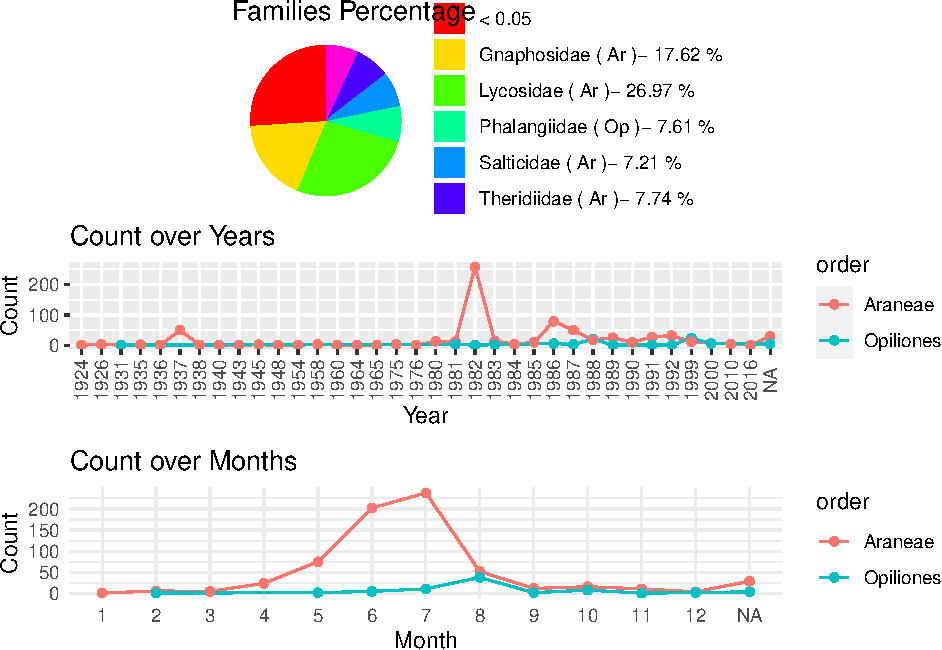
\includegraphics{Arachnida_files/figure-latex/groups.fig-1.pdf}
\caption{\label{fig:descrb}descrb}
\end{figure}

\begin{figure}
\centering
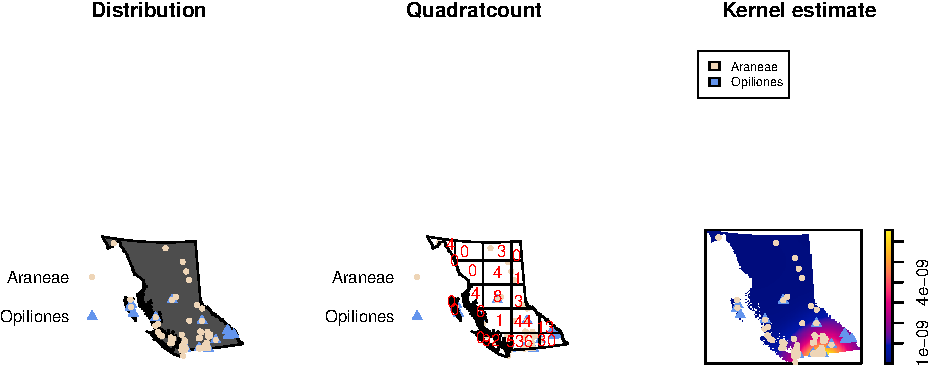
\includegraphics{Arachnida_files/figure-latex/Arachnida.Intensity.PLot-1.pdf}
\caption{\label{fig:intensity}Intensity Analysis}
\end{figure}

\begin{figure}
\centering
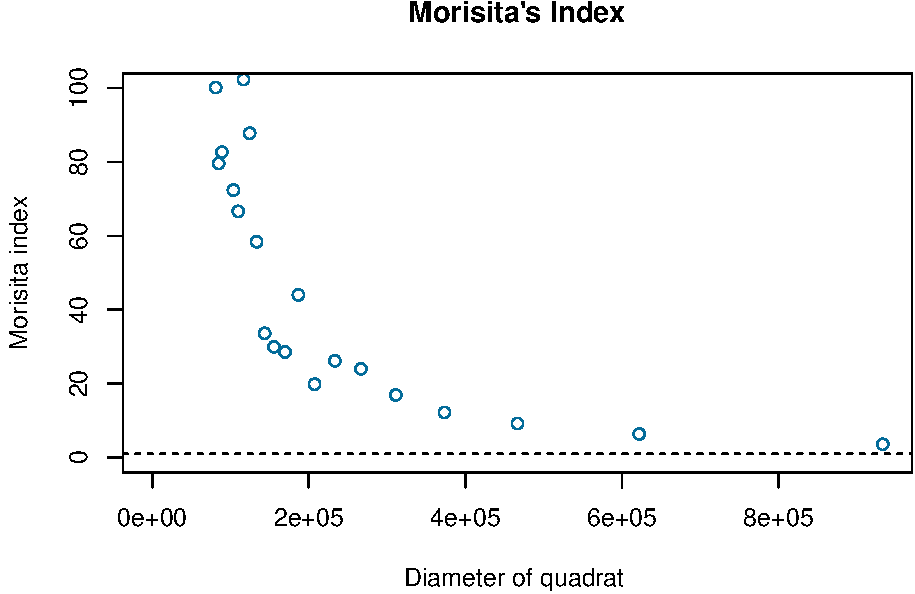
\includegraphics{Arachnida_files/figure-latex/Morisita-1.pdf}
\caption{\label{fig:Morisita}Morisita's Index}
\end{figure}

\begin{figure}
\centering
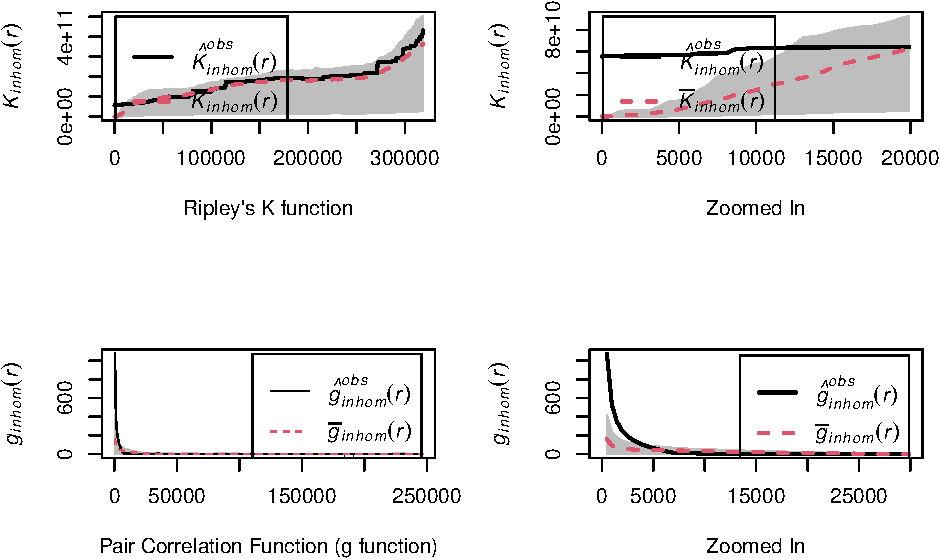
\includegraphics{Arachnida_files/figure-latex/KG.plot-1.pdf}
\caption{\label{fig:FandG}K Function and G Function}
\end{figure}

\begin{figure}
\centering
\includegraphics{Arachnida_files/figure-latex/Covariates-1.pdf}
\caption{\label{fig:covariates}Covariates}
\end{figure}

\begin{figure}
\centering
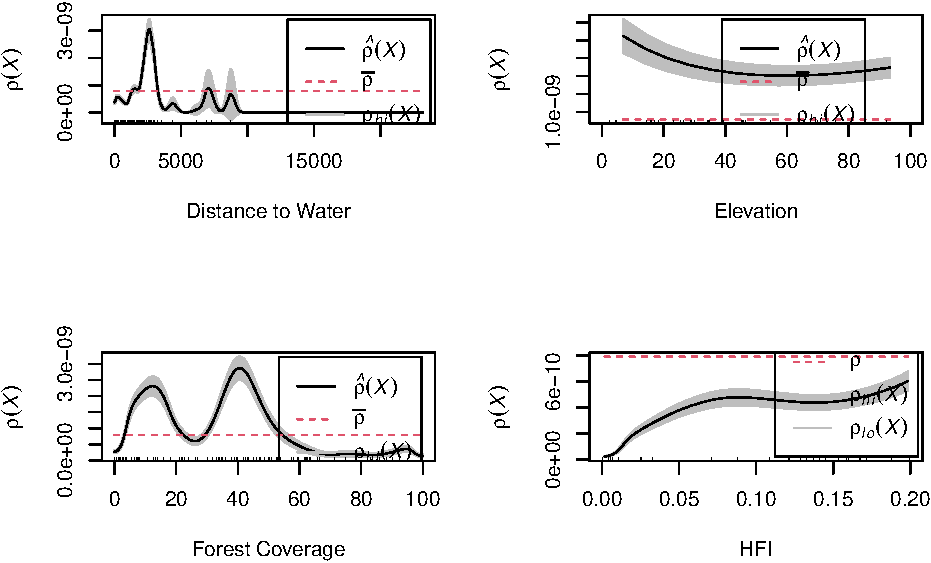
\includegraphics{Arachnida_files/figure-latex/Covariates.rela.fig-1.pdf}
\caption{\label{fig:CovKernek}Kernel Estimate for Covariates}
\end{figure}

\begin{figure}
\centering
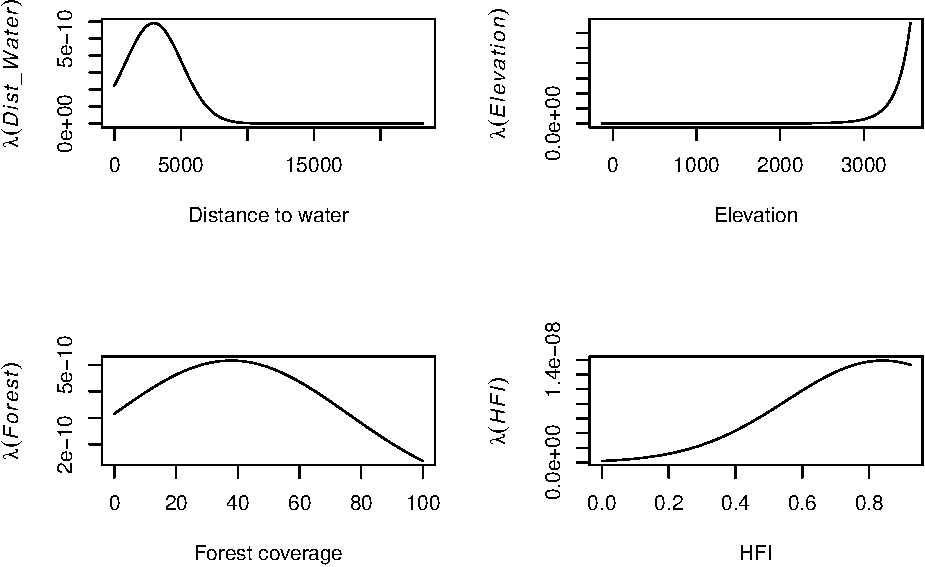
\includegraphics{Arachnida_files/figure-latex/ppm.effect-1.pdf}
\caption{\label{fig:effect} Covariate Effects at mean of other
covariates}
\end{figure}

\begin{figure}
\centering
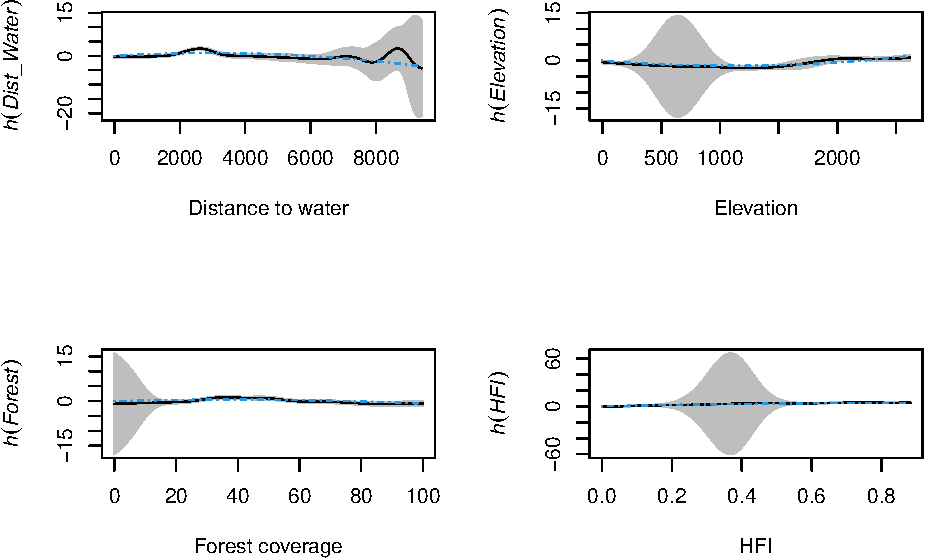
\includegraphics{Arachnida_files/figure-latex/res-1.pdf}
\caption{\label{fig:ResKernel}Partial Residual Plot}
\end{figure}

\bibliographystyle{unsrt}
\bibliography{references.bib}


\end{document}
